% !TeX root = ../Thesis.tex

%********************************************************************
% Notes on Installation and Usage (Appendix)
%*******************************************************
% If problems with the headers: get headings in appendix etc. right
%\markboth{\spacedlowsmallcaps{Appendix}}{\spacedlowsmallcaps{Appendix}}

%************************************************
\chapter{Additional Figures and Tables}\label{ch:AdditionalData}
%************************************************
\glsresetall % Resets all acronyms to not used

This Appendix provides additional figures and tables not directly referenced in this thesis, as well as larger versions of the individual plots presented in compact compound figures.

\section{Additional Tables}

\begin{table}[H]	
	\resizebox{\textwidth}{!}{
	\begin{tabular}{lllrrrrrrrr}
		\toprule
		&           & metric & \multicolumn{4}{l}{channel\_width} & \multicolumn{4}{l}{critical\_path} \\
		&           & attempt &             1 &     2 &     3 &   mean &             1 &     2 &     3 &  mean \\
		conv &  &  &               &       &       &        &               &       &       &       \\
		layer &  & kernel &               &       &       &        &               &       &       &       \\
		count & structure & size &               &       &       &        &               &       &       &       \\
		\midrule
		0 & deflating & -1 &          78.0 &  82.0 &  \textbf{80.0} &  80.00 &          6.65 &  6.12 &  \textbf{6.27} &  6.35 \\
		& inflating & -1 &          88.0 &  \textbf{80.0} &  80.0 &  82.67 &          6.74 &  \textbf{6.26} &  6.23 &  6.41 \\
		1 & deflating & 3 &          \textbf{78.0} &  78.0 &  80.0 &  78.67 &          7.53 &  6.84 &  \textbf{7.21} &  7.19 \\
		&           & 7 &          76.0 &  \textbf{78.0} &  80.0 &  78.00 &          8.02 &  6.11 &  \textbf{6.66} &  6.93 \\
		& inflating & 3 &          \textbf{82.0} &  80.0 &  84.0 &  82.00 &          6.57 &  7.16 &  \textbf{6.58} &  6.77 \\
		&           & 7 &          \textbf{78.0} &  76.0 &  80.0 &  78.00 &          6.00 &  \textbf{6.12} &  7.18 &  6.44 \\
		2 & deflating & 3 &          82.0 &  \textbf{80.0} &  78.0 &  80.00 &          \textbf{6.61} &  6.60 &  7.00 &  6.74 \\
		&           & 7 &          \textbf{80.0} &  84.0 &  80.0 &  81.33 &          7.83 &  \textbf{7.22} &  6.93 &  7.32 \\
		& inflating & 3 &          88.0 &  78.0 &  \textbf{80.0} &  82.00 &          7.49 &  6.24 &  \textbf{7.14} &  6.96 \\
		&           & 7 &          80.0 &  \textbf{78.0} &  78.0 &  78.67 &          6.58 &  7.28 &  \textbf{6.81} &  6.89 \\
		\bottomrule
	\end{tabular}
	}
	\caption{Full results of \gls{CNN} HPO. Median for each candidate marked in \textbf{bold}.}
\end{table}

\begin{table}[H]
	\resizebox{\textwidth}{!}{
	\begin{tabular}{lllrrrrrrrr}
		\toprule
		&   & metric & \multicolumn{4}{l}{channel\_width} & \multicolumn{4}{l}{critical\_path} \\
		&   & attempt &             1 &     2 &     3 &   mean &             1 &     2 &     3 &  mean \\
		lstm & dense &  &               &       &       &        &               &       &       &       \\
		layer & laye &  &               &       &       &        &               &       &       &       \\
		count & count & structure &               &       &       &        &               &       &       &       \\
		\midrule
		1 & 1 & bloating &          \textbf{78.0} &  80.0 &  78.0 &  78.67 &          \textbf{6.83} &  7.29 &  6.46 &  6.86 \\
		&   & deflating &          \textbf{80.0} &  88.0 &  80.0 &  82.67 &          6.54 &  \textbf{6.82} &  7.49 &  6.95 \\
		&   & inflating &          \textbf{78.0} &  78.0 &  78.0 &  78.00 &          \textbf{7.03} &  6.71 &  7.06 &  6.93 \\
		& 2 & bloating &          82.0 &  \textbf{80.0} &  78.0 &  80.00 &          \textbf{7.47} &  6.27 &  7.66 &  7.13 \\
		&   & deflating &          \textbf{78.0} &  78.0 &  80.0 &  78.67 &          7.47 &  6.72 &  \textbf{6.83} &  7.01 \\
		&   & inflating &          78.0 &  \textbf{80.0} &  84.0 &  80.67 &          7.00 &  \textbf{6.56} &  6.33 &  6.63 \\
		2 & 1 & bloating &          \textbf{80.0} &  84.0 &  78.0 &  80.67 &          \textbf{6.82} &  6.69 &  6.85 &  6.79 \\
		&   & deflating &          84.0 &  \textbf{82.0} &  82.0 &  82.67 &          7.01 &  \textbf{7.14} &  7.25 &  7.13 \\
		&   & inflating &          80.0 &  86.0 &  \textbf{82.0} &  82.67 &          8.50 &  6.94 &  \textbf{7.50} &  7.65 \\
		& 2 & bloating &          \textbf{84.0} &  84.0 &  80.0 &  82.67 &          6.67 &  7.83 &  \textbf{7.06} &  7.19 \\
		&   & deflating &          \textbf{82.0} &  84.0 &  80.0 &  82.00 &          6.53 &  \textbf{6.97} &  7.01 &  6.83 \\
		&   & inflating &          \textbf{78.0} &  78.0 &  80.0 &  78.67 &          7.21 &  6.64 &  \textbf{6.95} &  6.93 \\
		3 & 1 & bloating &          \textbf{84.0} &  84.0 &  88.0 &  85.33 &          \textbf{7.44} &  8.42 &  7.41 &  7.76 \\
		&   & deflating &          \textbf{84.0} &  86.0 &  84.0 &  84.67 &          \textbf{7.44} &  7.40 &  7.32 &  7.38 \\
		&   & inflating &          \textbf{86.0} &  84.0 &  86.0 &  85.33 &          \textbf{7.47} &  8.04 &  6.91 &  7.48 \\
		& 2 & bloating &          82.0 &  \textbf{86.0} &  88.0 &  85.33 &          8.26 &  \textbf{7.70} &  7.63 &  7.86 \\
		&   & deflating &          84.0 &  \textbf{86.0} &  90.0 &  86.67 &          9.78 &  7.38 &  \textbf{7.44} &  8.20 \\
		&   & inflating &          \textbf{86.0} &  86.0 &  86.0 &  86.00 &          6.68 &  \textbf{7.69} &  8.02 &  7.46 \\
		\bottomrule
	\end{tabular}
	}
	\caption{Full results of \gls{RNN} HPO. Median for each candidate marked in \textbf{bold}.}
\end{table}

\pagebreak
\section{Additional Figures}

\begin{figure}[H]
	\centering
	\begin{subfigure}[b]{0.49\linewidth}
		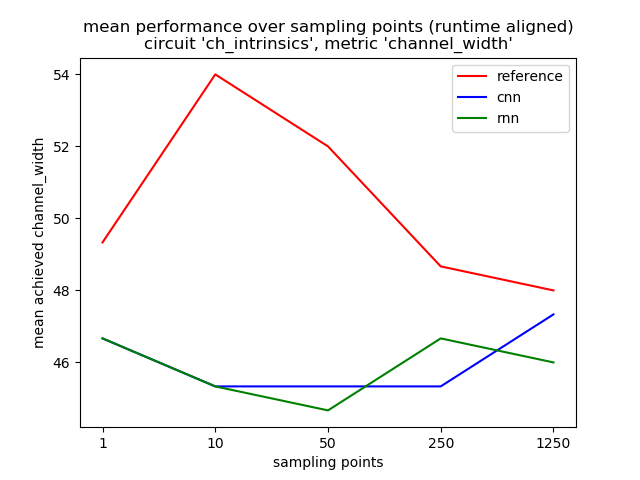
\includegraphics[width=\linewidth]{plots/eval-ch_intrinsics-chan-width-mean-full.png}
	\end{subfigure}
	\begin{subfigure}[b]{0.49\linewidth}
		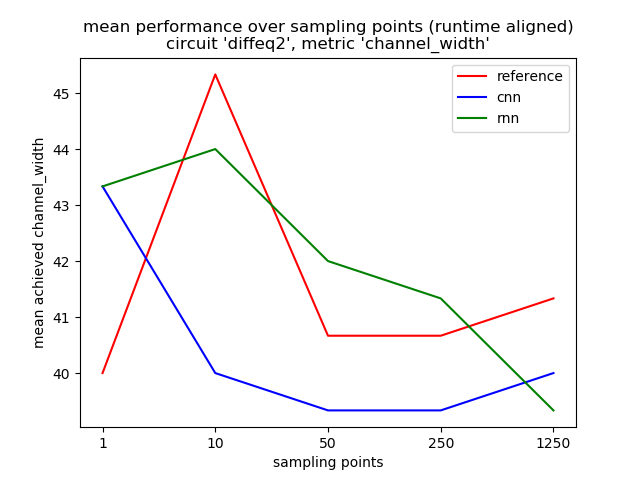
\includegraphics[width=\linewidth]{plots/eval-diffeq2-chan-width-mean-full.png}
	\end{subfigure}
	\begin{subfigure}[b]{0.49\linewidth}
		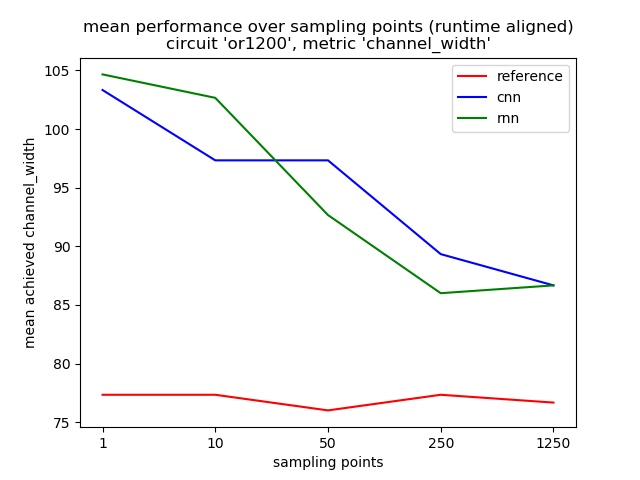
\includegraphics[width=\linewidth]{plots/eval-or1200-chan-width-mean-full.png}
	\end{subfigure}
	\begin{subfigure}[b]{0.49\linewidth}
		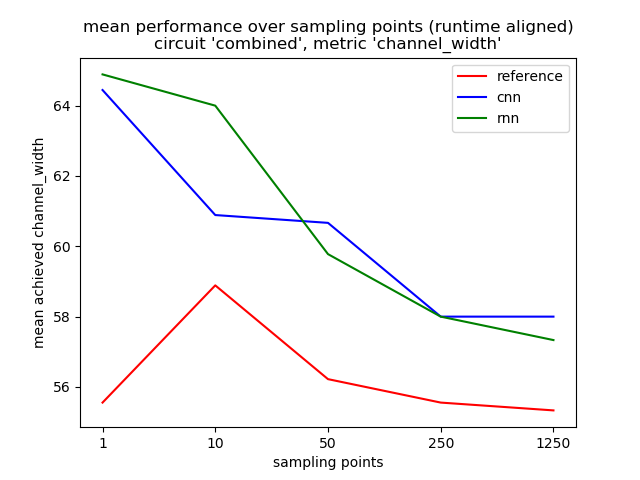
\includegraphics[width=\linewidth]{plots/eval-combined-chan-width-mean-full.png}
	\end{subfigure}
	\caption{Mean of achieved channel width over sampling points per circuit.}
	\label{fig:eval-chan-width-mean}
\end{figure}

\begin{figure}[H]
	\centering
	\begin{subfigure}[b]{0.49\linewidth}
		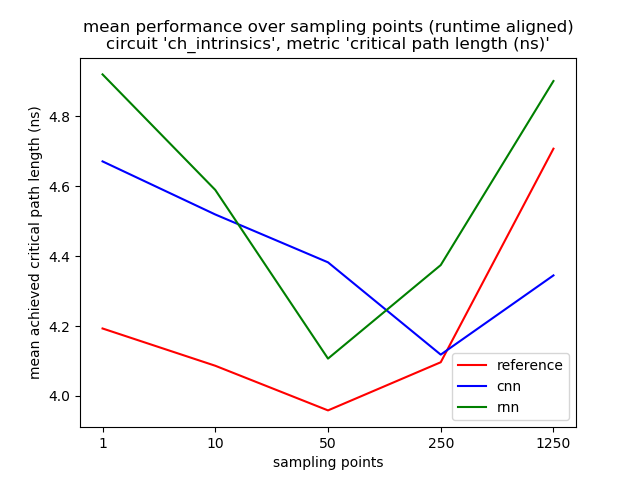
\includegraphics[width=\linewidth]{plots/eval-ch_intrinsics-critical-path-mean-full.png}
	\end{subfigure}
	\begin{subfigure}[b]{0.49\linewidth}
		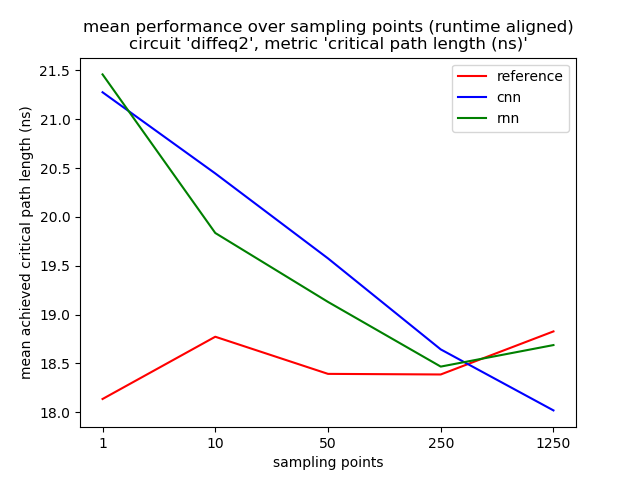
\includegraphics[width=\linewidth]{plots/eval-diffeq2-critical-path-mean-full.png}
	\end{subfigure}
	\begin{subfigure}[b]{0.49\linewidth}
		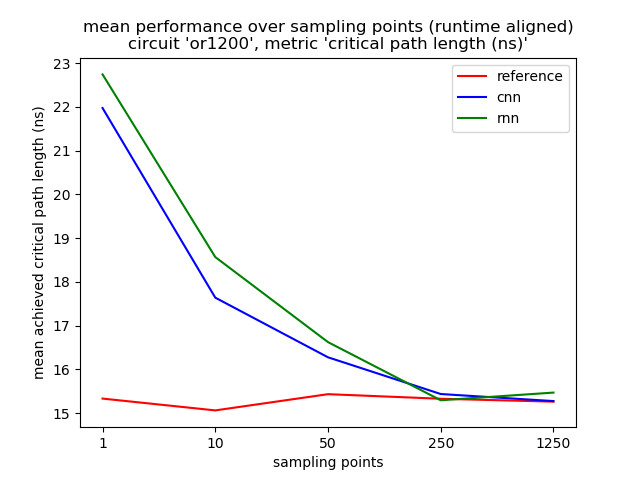
\includegraphics[width=\linewidth]{plots/eval-or1200-critical-path-mean-full.png}
	\end{subfigure}
	\begin{subfigure}[b]{0.49\linewidth}
		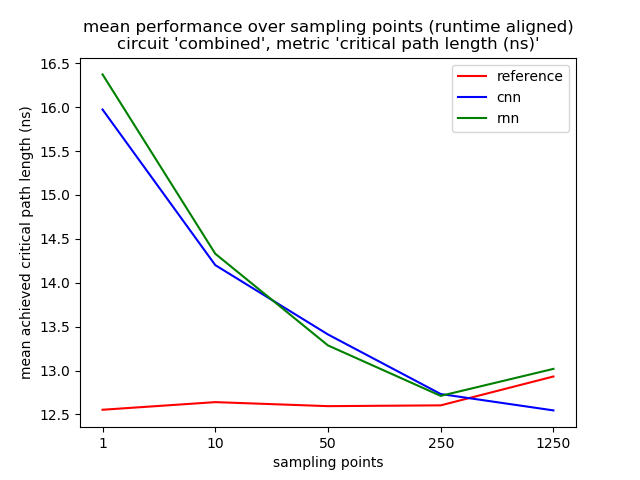
\includegraphics[width=\linewidth]{plots/eval-combined-critical-path-mean-full.png}
	\end{subfigure}
	\caption{Mean of achieved critical path length over sampling points per circuit.}
	\label{fig:eval-critical-path-mean}
\end{figure}

\begin{figure}[H]
	\centering
	\begin{subfigure}[b]{0.49\linewidth}
		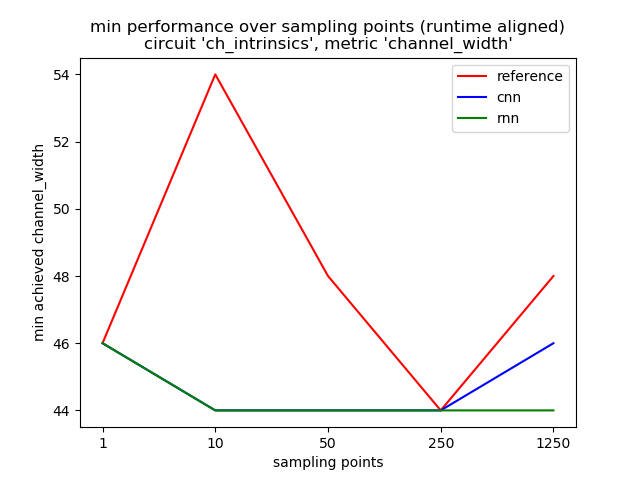
\includegraphics[width=\linewidth]{plots/eval-ch_intrinsics-chan-width-min-full.png}
	\end{subfigure}
	\begin{subfigure}[b]{0.49\linewidth}
		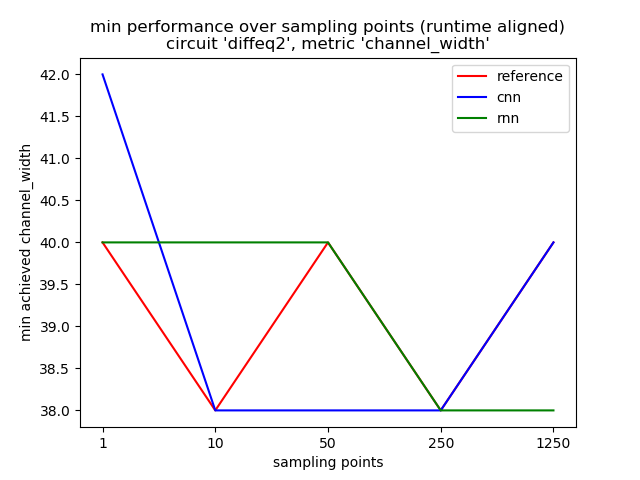
\includegraphics[width=\linewidth]{plots/eval-diffeq2-chan-width-min-full.png}
	\end{subfigure}
	\begin{subfigure}[b]{0.49\linewidth}
		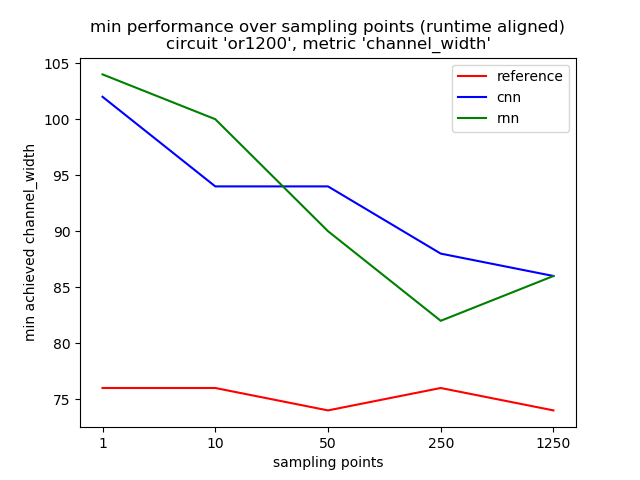
\includegraphics[width=\linewidth]{plots/eval-or1200-chan-width-min-full.png}
	\end{subfigure}
	\begin{subfigure}[b]{0.49\linewidth}
		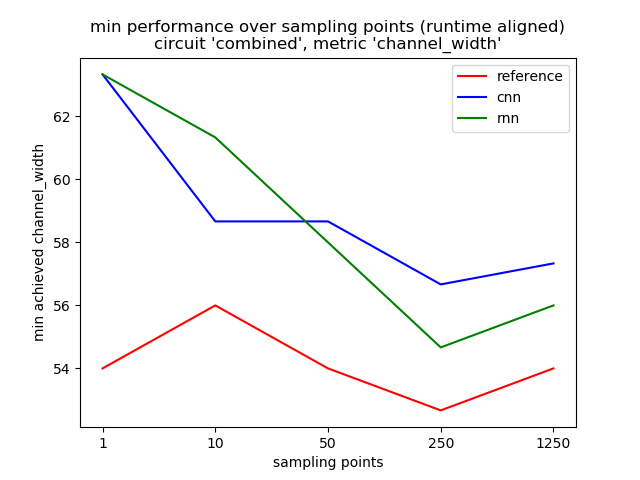
\includegraphics[width=\linewidth]{plots/eval-combined-chan-width-min-full.png}
	\end{subfigure}
	\caption{Minimum of achieved channel width over sampling points per circuit.}
	\label{fig:eval-chan-width-min}
\end{figure}

\begin{figure}[H]
	\centering
	\begin{subfigure}[b]{0.49\linewidth}
		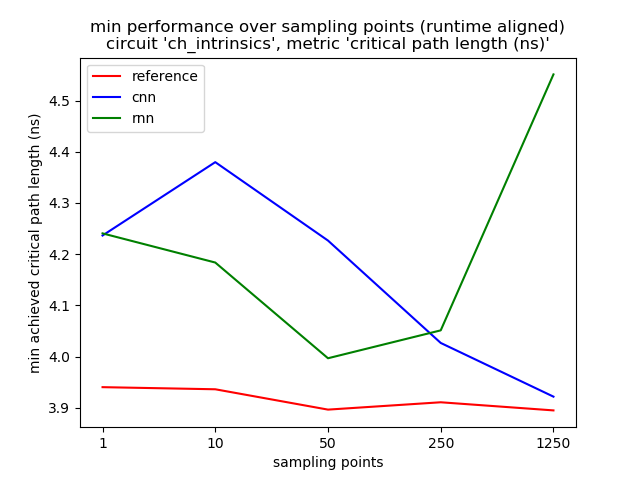
\includegraphics[width=\linewidth]{plots/eval-ch_intrinsics-critical-path-min-full.png}
	\end{subfigure}
	\begin{subfigure}[b]{0.49\linewidth}
		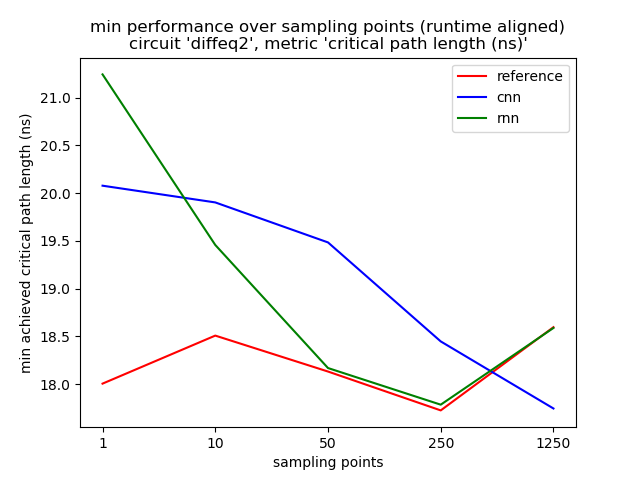
\includegraphics[width=\linewidth]{plots/eval-diffeq2-critical-path-min-full.png}
	\end{subfigure}
	\begin{subfigure}[b]{0.49\linewidth}
		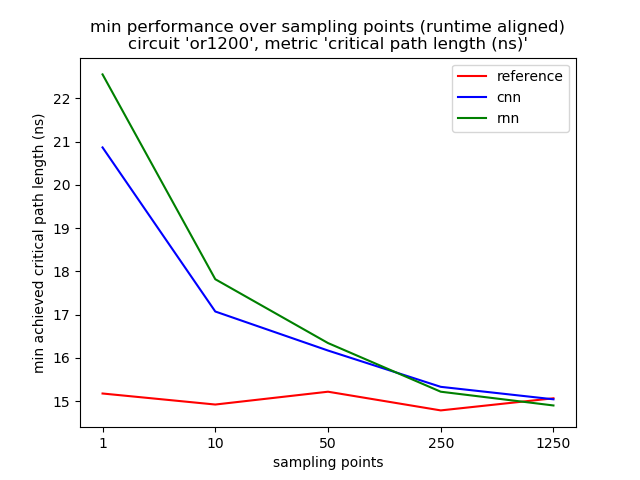
\includegraphics[width=\linewidth]{plots/eval-or1200-critical-path-min-full.png}
	\end{subfigure}
	\begin{subfigure}[b]{0.49\linewidth}
		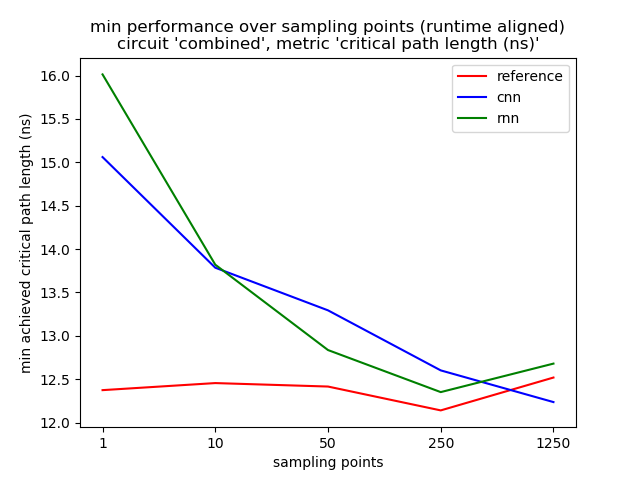
\includegraphics[width=\linewidth]{plots/eval-combined-critical-path-min-full.png}
	\end{subfigure}
	\caption{Minimum of achieved critical path length over sampling points per circuit.}
	\label{fig:eval-critical-path-min}
\end{figure}

\let\svaddcontentsline\addcontentsline
\renewcommand\addcontentsline[3]{%
	\edef\qtest{#1}%
	\def\qmatch{lof}%
	\ifx\qmatch\qtest\else%
	\def\qmatch{lot}%
	\ifx\qmatch\qtest\else%
	\svaddcontentsline{#1}{#2}{#3}%
	\fi\fi%
}

\pagebreak
\section{Individual Full-Size Figures}

Full size figures are labelled by their position in the original compound plot and the corresponding figure reference. This enables easy lookup of a certain plot, while its description can be accessed by following the reference to the compound plot.

\subsection{Training Data Histograms}

\begin{figure}[H]
	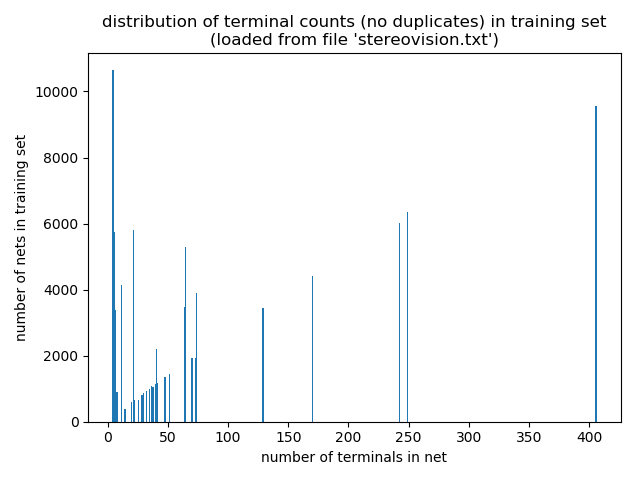
\includegraphics[width=\linewidth]{plots/data-distribution-full-fine.png}
	\caption{Figure \ref{fig:data-hist}, top left}
\end{figure}

\begin{figure}[H]
	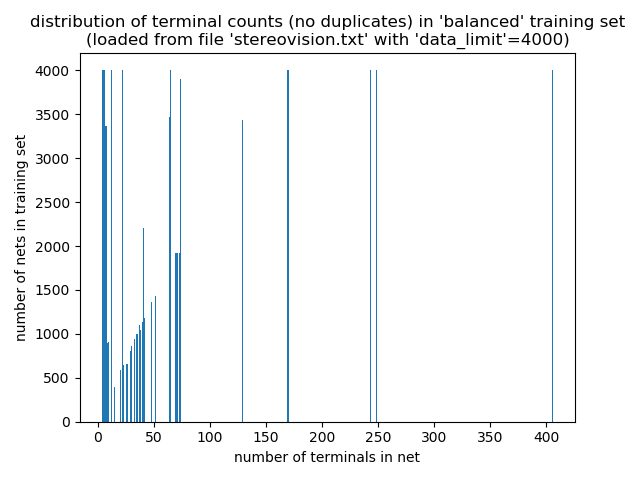
\includegraphics[width=\linewidth]{plots/data-distribution-limited-fine.png}
	\caption{Figure \ref{fig:data-hist}, top right}
\end{figure}

\begin{figure}[H]
	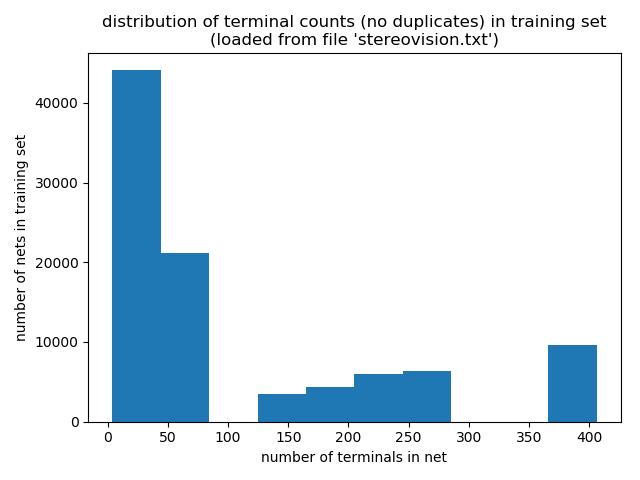
\includegraphics[width=\linewidth]{plots/data-distribution-full-coarse.png}
	\caption{Figure \ref{fig:data-hist}, bottom left}
\end{figure}

\begin{figure}[H]
	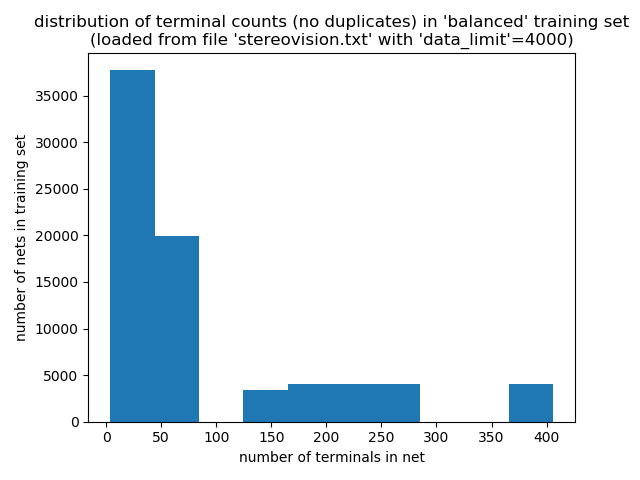
\includegraphics[width=\linewidth]{plots/data-distribution-limited-coarse.png}
	\caption{Figure \ref{fig:data-hist}, bottom right}
\end{figure}

\subsection{Training Histories}

\begin{figure}[H]
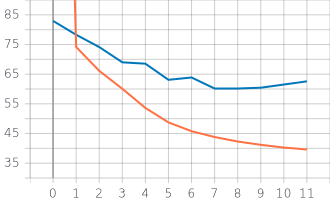
\includegraphics[width=\linewidth]{plots/cnn-training-history-2_conv_layers_deflating_kernel_size_7.png}
\caption{Figure \ref{fig:cnn-train}, left}
\end{figure}

\begin{figure}[H]
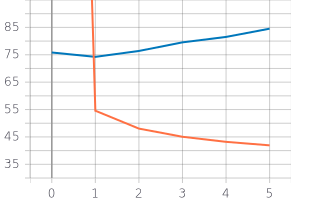
\includegraphics[width=\linewidth]{plots/cnn-training-history-1_conv_layers_deflating_kernel_size_7.png}
\caption{Figure \ref{fig:cnn-train}, middle}
\end{figure}

\begin{figure}[H]
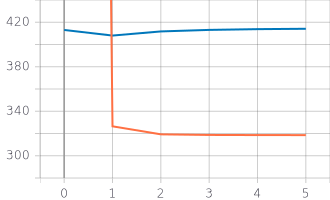
\includegraphics[width=\linewidth]{plots/cnn-training-history-0_conv_layers_deflating_kernel_size_-1.png}
\caption{Figure \ref{fig:cnn-train}, right}
\end{figure}

\begin{figure}[H]
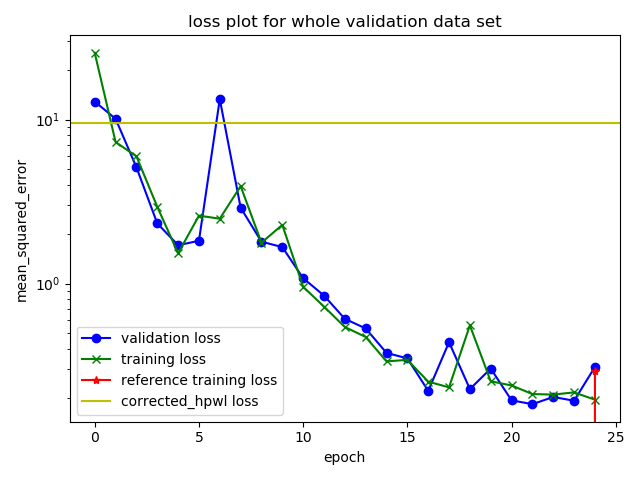
\includegraphics[width=\linewidth]{plots/rnn-training-history-3_lstm_layers_2_dense_layers_inflating.png}
\caption{TODO Figure \ref{fig:rnn-training}, left}
\end{figure}

\begin{figure}[H]
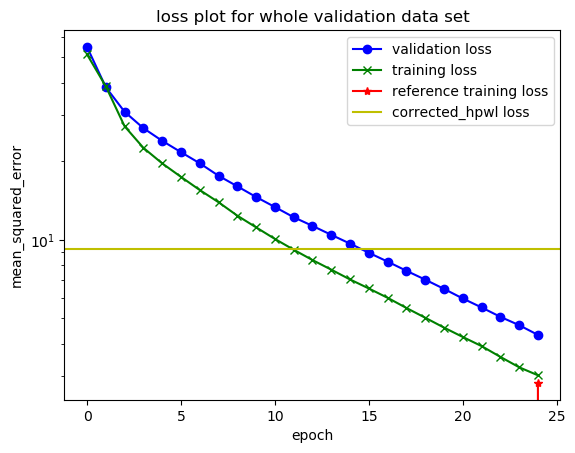
\includegraphics[width=\linewidth]{plots/rnn-training-history-1_lstm_layers_1_dense_layers_inflating.png}
\caption{Figure \ref{fig:rnn-training}, right}
\end{figure}

\subsection{\gls{HPO}}

\begin{figure}[H]
	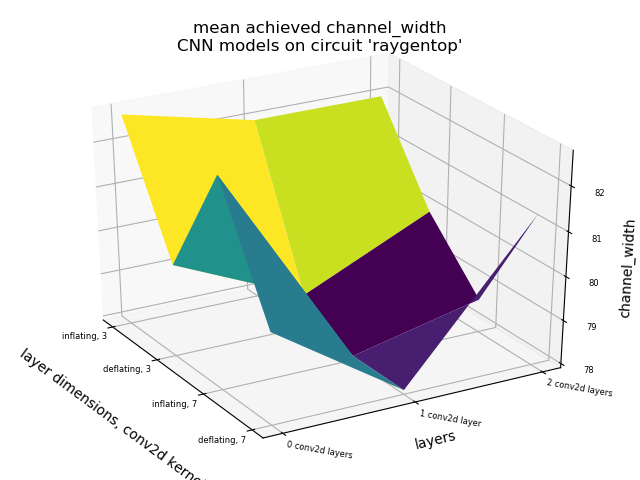
\includegraphics[width=\linewidth]{plots/cnn-hyperopt-chan-width.png}
	\caption{Figure \ref{fig:eval-hyperopt-surface}, top left}
\end{figure}

\begin{figure}[H]
	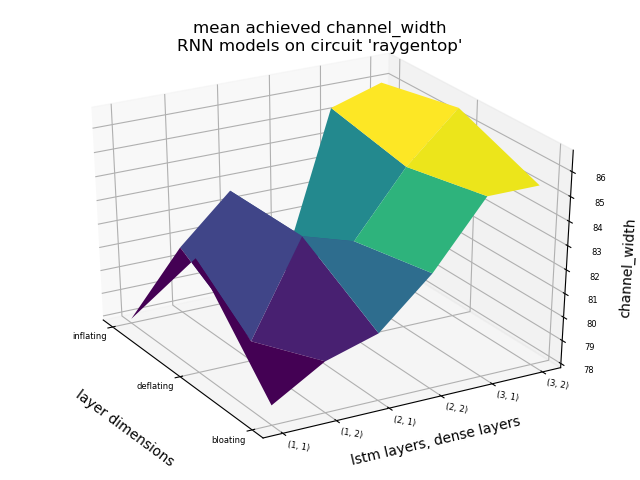
\includegraphics[width=\linewidth]{plots/rnn-hyperopt-chan-width.png}
	\caption{Figure \ref{fig:eval-hyperopt-surface}, top right}
\end{figure}

\begin{figure}[H]
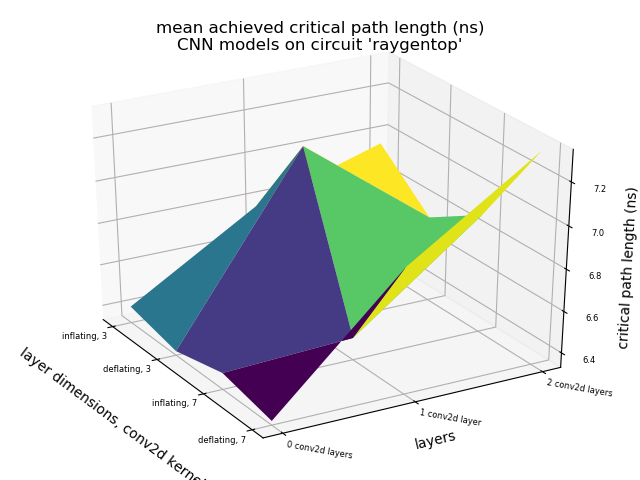
\includegraphics[width=\linewidth]{plots/cnn-hyperopt-critical-path.png}
\caption{Figure \ref{fig:eval-hyperopt-surface}, bottom left}
\end{figure}

\begin{figure}[H]
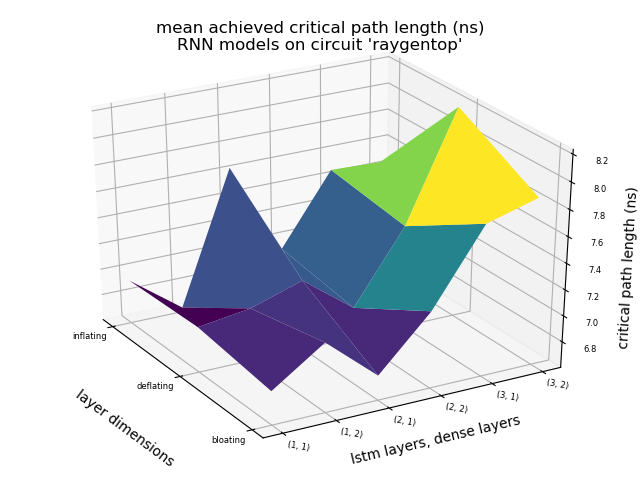
\includegraphics[width=\linewidth]{plots/rnn-hyperopt-critical-path.png}
\caption{Figure \ref{fig:eval-hyperopt-surface}, bottom right}
\end{figure}

\begin{figure}[H]
	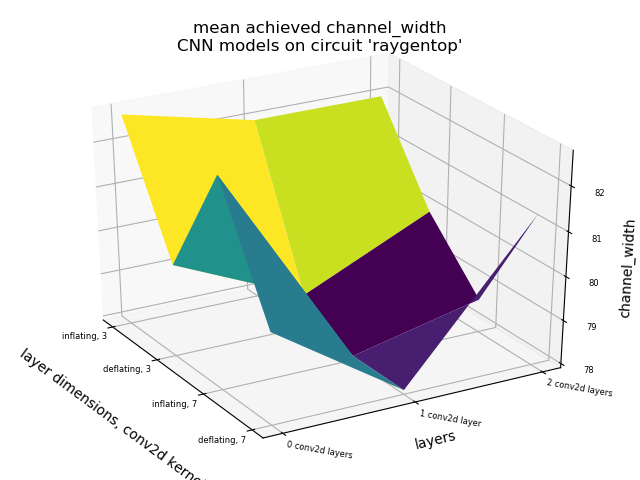
\includegraphics[width=\linewidth]{plots/cnn-hyperopt-chan-width.png}
	\caption{Figure \ref{fig:eval-hyperopt-surface-reference}, top left}
\end{figure}

\begin{figure}[H]
	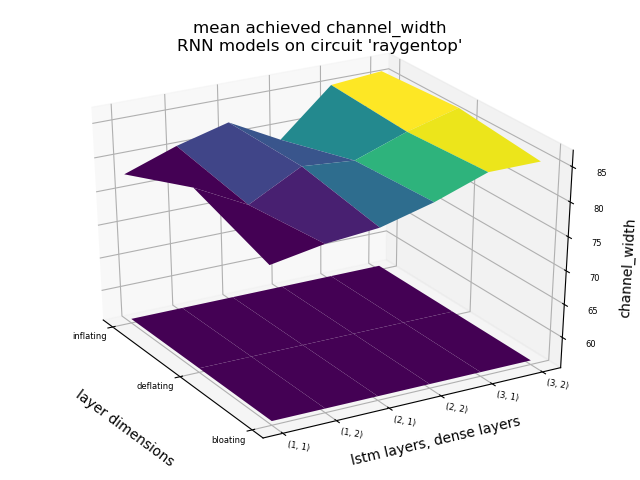
\includegraphics[width=\linewidth]{plots/rnn-hyperopt-chan-width-with-reference.png}
	\caption{Figure \ref{fig:eval-hyperopt-surface-reference}, top right}
\end{figure}

\begin{figure}[H]
	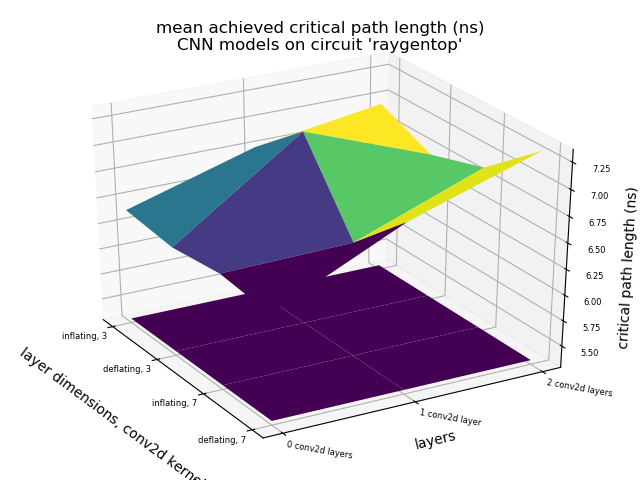
\includegraphics[width=\linewidth]{plots/cnn-hyperopt-critical-path-with-reference.png}
	\caption{Figure \ref{fig:eval-hyperopt-surface-reference}, bottom left}
\end{figure}

\begin{figure}[H]
	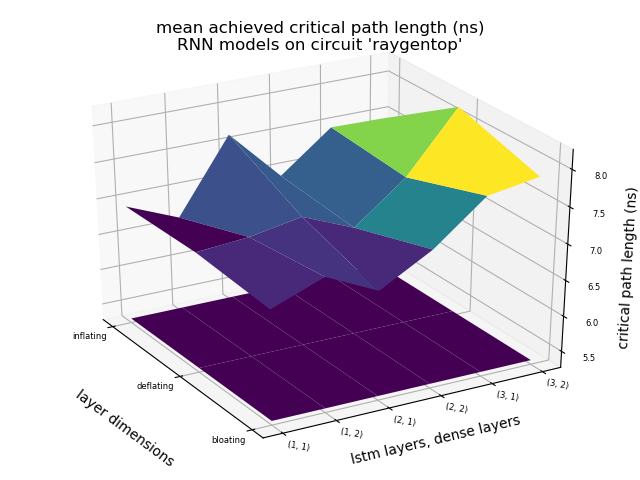
\includegraphics[width=\linewidth]{plots/rnn-hyperopt-critical-path-with-reference.png}
	\caption{Figure \ref{fig:eval-hyperopt-surface-reference}, bottom right}
\end{figure}

\subsection{Final Evaluation Results}

\begin{figure}[H]
	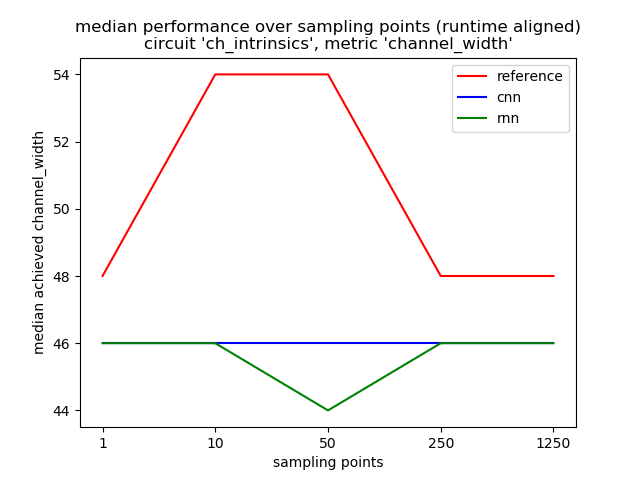
\includegraphics[width=\linewidth]{plots/eval-ch_intrinsics-chan-width-median-full.png}
	\caption{Figure \ref{fig:eval-chan-width-median}, top left}
\end{figure}

\begin{figure}[H]
	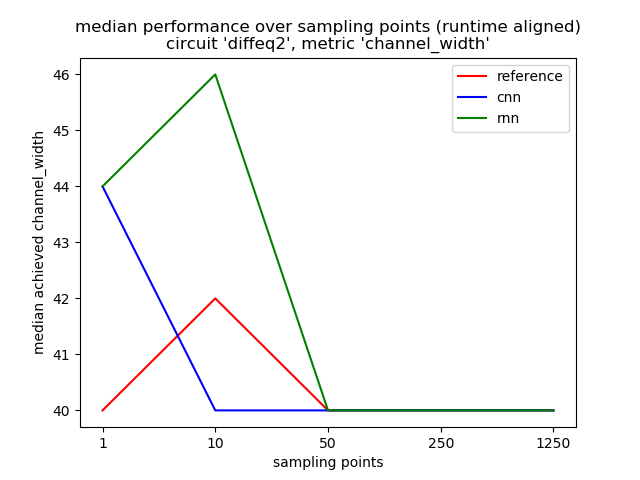
\includegraphics[width=\linewidth]{plots/eval-diffeq2-chan-width-median-full.png}
	\caption{Figure \ref{fig:eval-chan-width-median}, top right}
\end{figure}

\begin{figure}[H]
	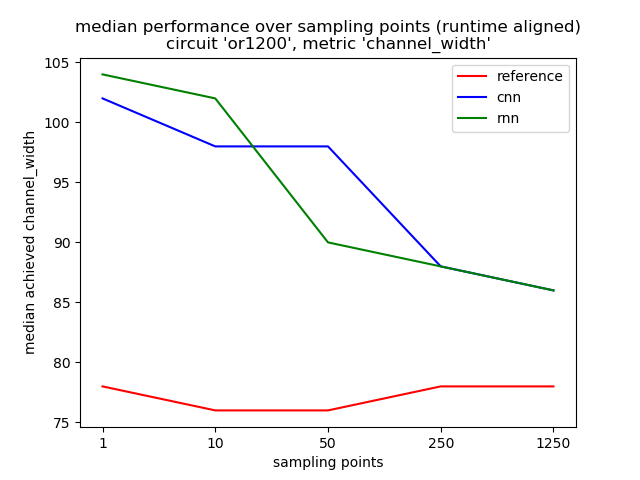
\includegraphics[width=\linewidth]{plots/eval-or1200-chan-width-median-full.png}
	\caption{Figure \ref{fig:eval-chan-width-median}, bottom left}
\end{figure}

\begin{figure}[H]
	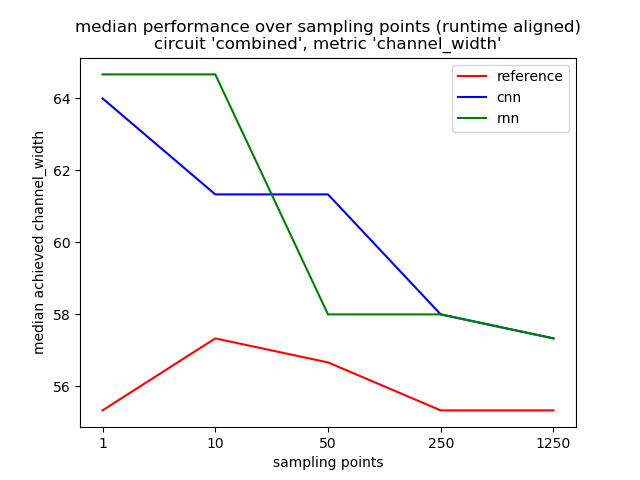
\includegraphics[width=\linewidth]{plots/eval-combined-chan-width-median-full.png}
	\caption{Figure \ref{fig:eval-chan-width-median}, bottom right}
\end{figure}

\begin{figure}[H]
	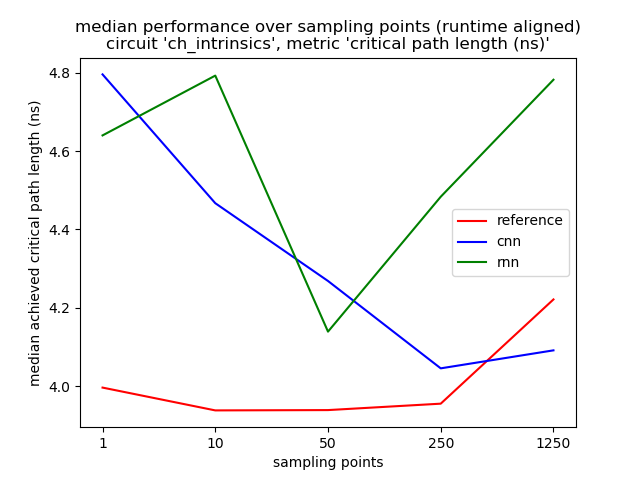
\includegraphics[width=\linewidth]{plots/eval-ch_intrinsics-critical-path-median-full.png}
	\caption{Figure \ref{fig:eval-critical-path-median}, top left}
\end{figure}

\begin{figure}[H]
	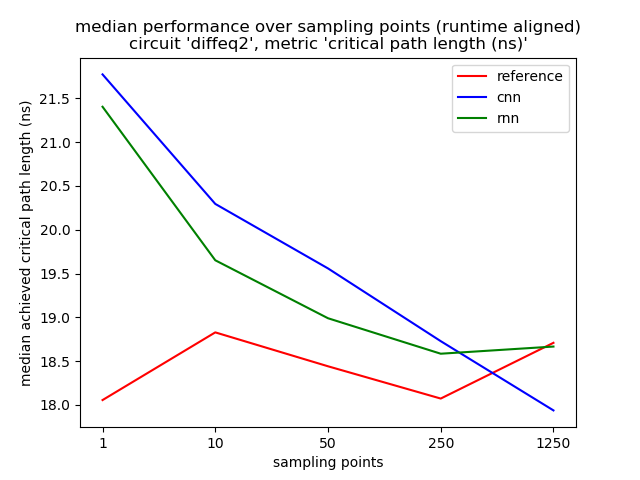
\includegraphics[width=\linewidth]{plots/eval-diffeq2-critical-path-median-full.png}
	\caption{Figure \ref{fig:eval-critical-path-median}, top right}
\end{figure}

\begin{figure}[H]
	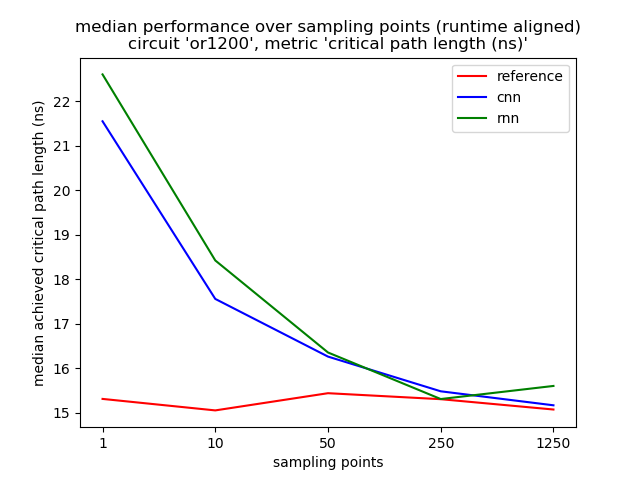
\includegraphics[width=\linewidth]{plots/eval-or1200-critical-path-median-full.png}
	\caption{Figure \ref{fig:eval-critical-path-median}, bottom left}
\end{figure}

\begin{figure}[H]
	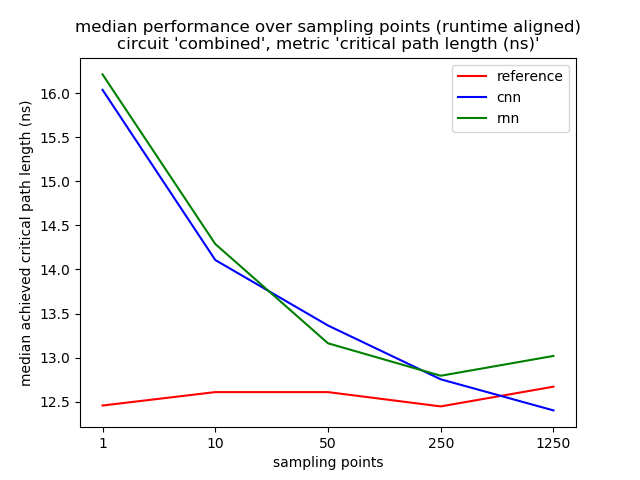
\includegraphics[width=\linewidth]{plots/eval-combined-critical-path-median-full.png}
	\caption{Figure \ref{fig:eval-critical-path-median}, bottom right}
\end{figure}

\begin{figure}[H]
	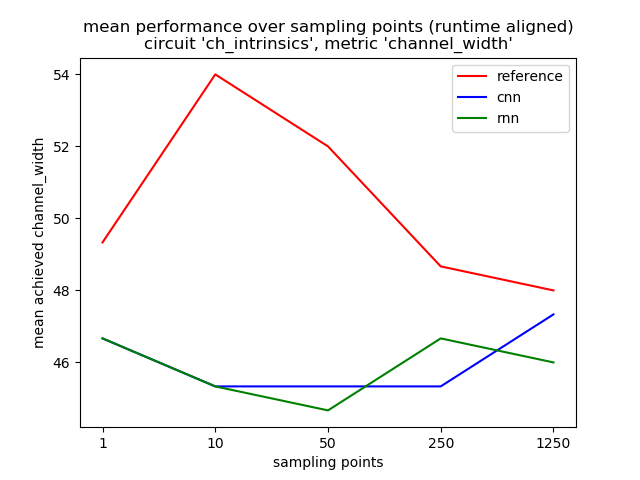
\includegraphics[width=\linewidth]{plots/eval-ch_intrinsics-chan-width-mean-full.png}
	\caption{Figure \ref{fig:eval-chan-width-mean}, top left}
\end{figure}

\begin{figure}[H]
	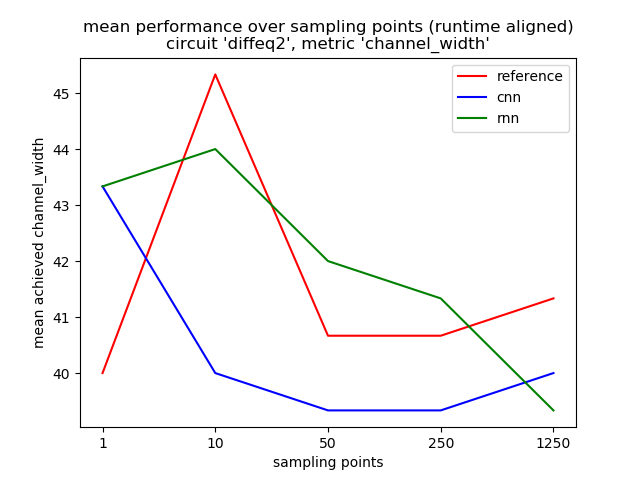
\includegraphics[width=\linewidth]{plots/eval-diffeq2-chan-width-mean-full.png}
	\caption{Figure \ref{fig:eval-chan-width-mean}, top right}
\end{figure}

\begin{figure}[H]
	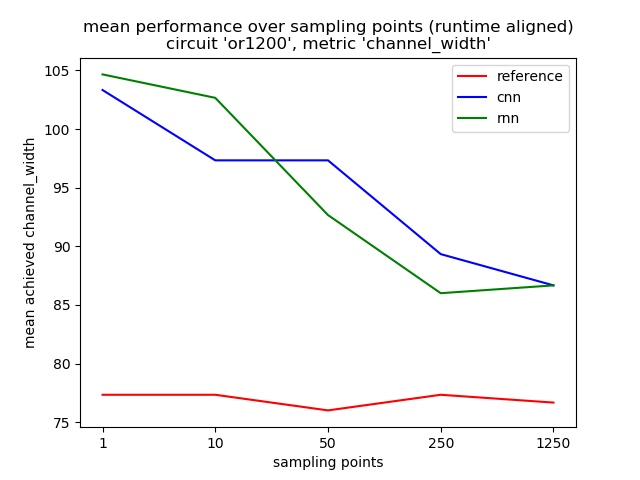
\includegraphics[width=\linewidth]{plots/eval-or1200-chan-width-mean-full.png}
	\caption{Figure \ref{fig:eval-chan-width-mean}, bottom left}
\end{figure}

\begin{figure}[H]
	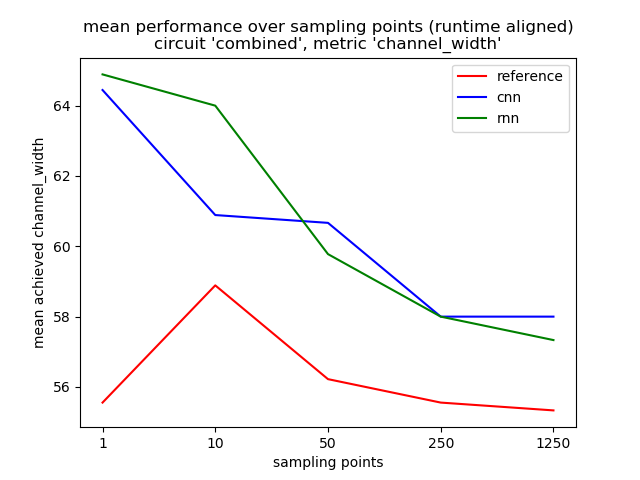
\includegraphics[width=\linewidth]{plots/eval-combined-chan-width-mean-full.png}
	\caption{Figure \ref{fig:eval-chan-width-mean}, bottom right}
\end{figure}

\begin{figure}[H]
	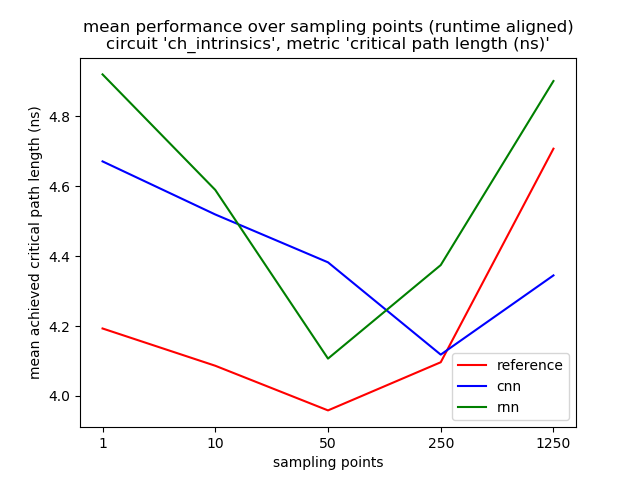
\includegraphics[width=\linewidth]{plots/eval-ch_intrinsics-critical-path-mean-full.png}
	\caption{Figure \ref{fig:eval-critical-path-mean}, top left}
\end{figure}

\begin{figure}[H]
	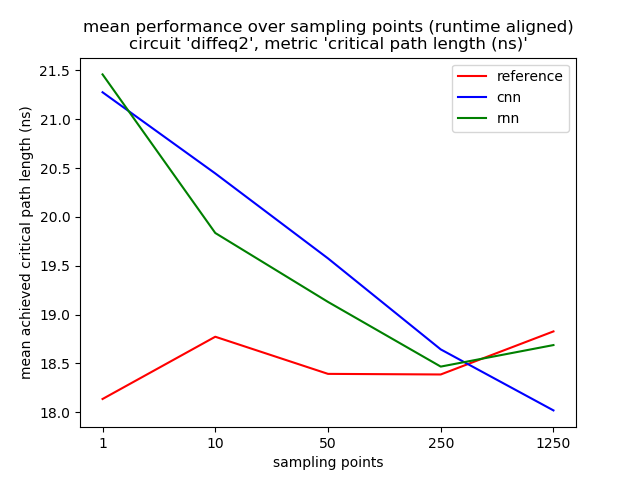
\includegraphics[width=\linewidth]{plots/eval-diffeq2-critical-path-mean-full.png}
	\caption{Figure \ref{fig:eval-critical-path-mean}, top right}
\end{figure}

\begin{figure}[H]
	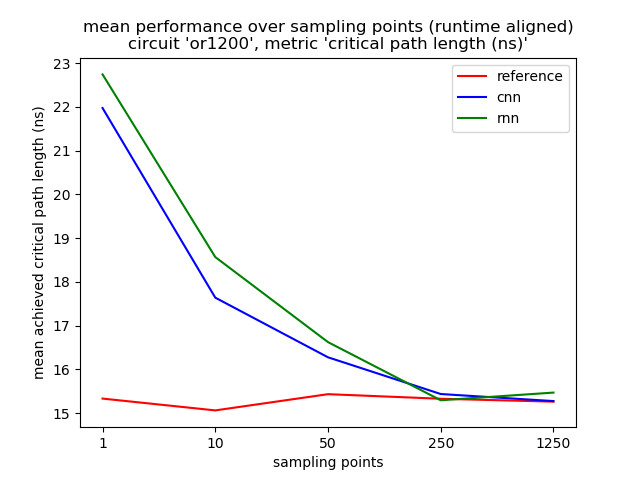
\includegraphics[width=\linewidth]{plots/eval-or1200-critical-path-mean-full.png}
	\caption{Figure \ref{fig:eval-critical-path-mean}, bottom left}
\end{figure}

\begin{figure}[H]
	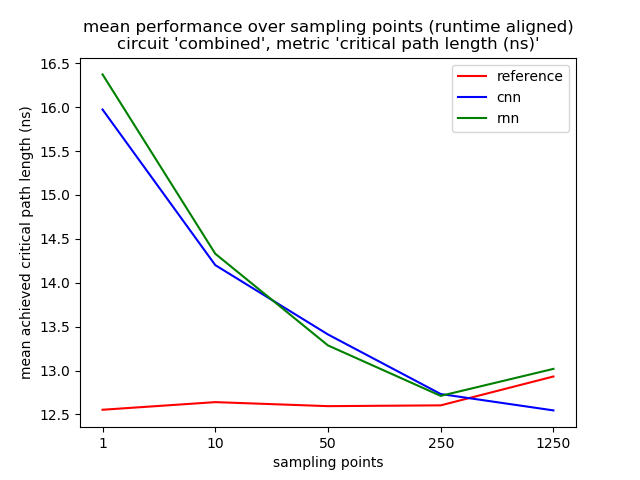
\includegraphics[width=\linewidth]{plots/eval-combined-critical-path-mean-full.png}
	\caption{Figure \ref{fig:eval-critical-path-mean}, bottom right}
\end{figure}

\begin{figure}[H]
	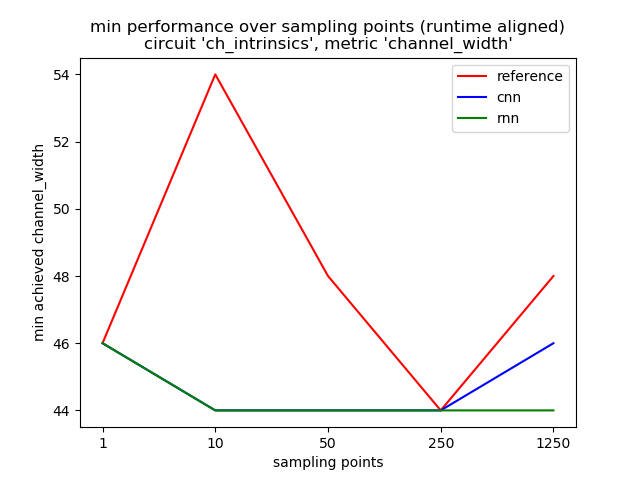
\includegraphics[width=\linewidth]{plots/eval-ch_intrinsics-chan-width-min-full.png}
	\caption{Figure \ref{fig:eval-chan-width-min}, top left}
\end{figure}

\begin{figure}[H]
\includegraphics[width=\linewidth]{plots/eval-diffeq2-chan-width-min-full.png}
\caption{Figure \ref{fig:eval-chan-width-min}, top right}
\end{figure}

\begin{figure}[H]
\includegraphics[width=\linewidth]{plots/eval-or1200-chan-width-min-full.png}
\caption{Figure \ref{fig:eval-chan-width-min}, bottom left}
\end{figure}

\begin{figure}[H]
\includegraphics[width=\linewidth]{plots/eval-combined-chan-width-min-full.png}
\caption{Figure \ref{fig:eval-chan-width-min}, bottom right}
\end{figure}

\begin{figure}[H]
\includegraphics[width=\linewidth]{plots/eval-ch_intrinsics-critical-path-min-full.png}
\caption{Figure \ref{fig:eval-critical-path-min}, top left}
\end{figure}

\begin{figure}[H]
\includegraphics[width=\linewidth]{plots/eval-diffeq2-critical-path-min-full.png}
\caption{Figure \ref{fig:eval-critical-path-min}, top right}
\end{figure}

\begin{figure}[H]
\includegraphics[width=\linewidth]{plots/eval-or1200-critical-path-min-full.png}
\caption{Figure \ref{fig:eval-critical-path-min}, bottom left}
\end{figure}

\begin{figure}[H]
\includegraphics[width=\linewidth]{plots/eval-combined-critical-path-min-full.png}
\caption{Figure \ref{fig:eval-critical-path-min}, bottom right}
\end{figure}